\chapter{Specifikacija programske potpore}
		
	\section{Funkcionalni zahtjevi}
			
		
			
			
			\noindent \textbf{Dionici:}
			
			\begin{packed_enum}
				
				\item Korisnici aplikacije
				\item Klijenti aplikacije				
				\item Zaposlenici aplikacije
					\begin{packed_enum}
					
					\item Trener
					\item Članovi uprave
					\end{packed_enum}
				\item Administrator
				\item Razvojni tim
				
				
			\end{packed_enum}
			
			\noindent \textbf{Aktori i njihovi funkcionalni zahtjevi:}
			
			
			\begin{packed_enum}
				\item  \underbar{Neregistrirani/Neprijavljeni korisnik(inicijator) može:}
				
				\begin{packed_enum}
					
					\item pregledavati sadržaj web aplikacije
					\item dodavati artikle u košaricu web shop-a, brisati jedan ili sve, pregledavati košaricu
					\item registrirati se, tj. napraviti novi korisnički račun s potrebnim podacima
					\item promijeniti jezik aplikacije				
				\end{packed_enum}
			
				\item  \underbar{Klijent aplikacije može:}
				
				\begin{packed_enum}
					
					\item sve što može neregistrirani korisnik osim registracije
					\item pregledavati i mijenjati osobne podatke
					\item izbrisati svoj korisnički račun
					\item platiti narudžbu
					\item ostaviti recenziju na web shop-u
					\item koristiti prijenos utakmica uživo
					\item koristiti chat uslugu pri gledanju prijenosa uživo
					
				\end{packed_enum}
			\item  \underbar{Trener, odnosno upravitelj kluba (inicijator) može:}
			
			\begin{packed_enum}
				
				\item dodavati sadržaj na stranicu, brisati ili mijenjati postojeći
				\item dodati novog igrača
				\item promijeniti podatke postojećem igraču
				\item izbrisati igrača iz kluba
				
			\end{packed_enum}
		\item  \underbar{Član uprave (inicijator) može:}
		
		\begin{packed_enum}
			
			\item pregledati aktivne narudžbe
			\item označiti narudžbu zaprimljenom
			\item uređivati artikle na web shop-u
			\item dodati artikl u web shop
			\item dodati popuste na web shop
			
		\end{packed_enum}
	
	\item  \underbar{Aministrator aplikacije (inicijator) može:}
	
	\begin{packed_enum}
		
		\item dodavati nove račune (trenera, administratora i upravu)
		\item brisati račune
		\item brisati recenzije
		\item pregledavati klijente
		\item promijeniti prava pristupa
	
	\end{packed_enum}
\item  \underbar{Baza podataka (sudionik):}

\begin{packed_enum}
	
	\item pohranjuje sve podatke o korisnicima i njihovim ovlastima
	\item pohranjuje sve podatke o sadržaju, ponudi i količinama

	
\end{packed_enum}
		\item  \underbar{Banka (sudionik):}
		
		\begin{packed_enum}
			
			\item provjerava, odnosno vrši transakcije prilikom plaćanja u web shop-u
			
			
		\end{packed_enum}
			\end{packed_enum}
			
			\eject 
			
			
				
			\subsection{Obrasci uporabe}
				
				
					

					\noindent \underbar{\textbf{UC1: Pregled web stranice}}
					\begin{packed_item}
	
						\item \textbf{Glavni sudionik: } Korisnik, klijent
						\item  \textbf{Cilj:} Pregledati sadržaj web stranice, uključujući web shop
						\item  \textbf{Sudionici:} Baza podataka
						\item  \textbf{Preduvjet:} -
						\item  \textbf{Opis osnovnog tijeka:}
						
						\item[] \begin{packed_enum}
	
							\item Stranica je prikazana tijekom pokretanja aplikacije
							\item Korisnik ili klijent pregledava sadržaj (Kontak, O nama, ...)
						\end{packed_enum}
						
				
						\end{packed_item}
					
					\noindent \underbar{\textbf{UC2: Registracija}}
					\begin{packed_item}
						
						\item \textbf{Glavni sudionik: } Korisnik
						\item  \textbf{Cilj:} Stvoriti korisnički račun
						\item  \textbf{Sudionici:} Baza podataka
						\item  \textbf{Preduvjet:} -
						\item  \textbf{Opis osnovnog tijeka:}
						
						\item[] \begin{packed_enum}
							
							\item Korisnik odabire opciju za registraciju
							\item Korisnik unosi podatke potrebne za registraciju
							\item Korisnik dobiva obavijest o uspješnoj registraciji
						\end{packed_enum}
						
						\item  \textbf{Opis mogućih odstupanja:}
						
						\item[] \begin{packed_item}
							
							\item[2.a] Odabir već zauzetog korisničkog imena ili e-maila, unos korisničkog podatka u nedozvoljenom formatu ili pružanje neispravnoga e-maila
							
							\item[] \begin{packed_enum}
								
								\item Sustav obavještava korisnika o neuspjelom upisu
								\item Korisnik mijenja potrebne podatke te završava unos ili odustaje od registracije
								
								
							\end{packed_enum}
							
						\end{packed_item}
					\end{packed_item}
				
				\noindent \underbar{\textbf{UC3: Prijava u sustav}}
				\begin{packed_item}
					
					\item \textbf{Glavni sudionik: } Klijent
					\item  \textbf{Cilj:} Dobiti pristup sustavu
					\item  \textbf{Sudionici:} Baza podataka
					\item  \textbf{Preduvjet:} Registracija
					\item  \textbf{Opis osnovnog tijeka:}
					
					\item[] \begin{packed_enum}
						
						\item Korisnik odabire opciju za prijavu
						\item Korisnik unosi podatke potrebne za prijavu (korisničko ime i lozinka)
						\item Korisnik dobiva pristup korisničkim funkcijama
					\end{packed_enum}
					
					\item  \textbf{Opis mogućih odstupanja:}
					
					\item[] \begin{packed_item}
						
						\item[2.a] Neispravno korisničko ime ili lozinka
						
						\item[] \begin{packed_enum}
							
							\item Sustav obavještava korisnika o neuspjelom upisu

							
							
						\end{packed_enum}
						
					\end{packed_item}
				\end{packed_item}
					
					
					
				
				
					
				\subsubsection{Dijagrami obrazaca uporabe}
					
				
					
					\begin{figure}[H]
						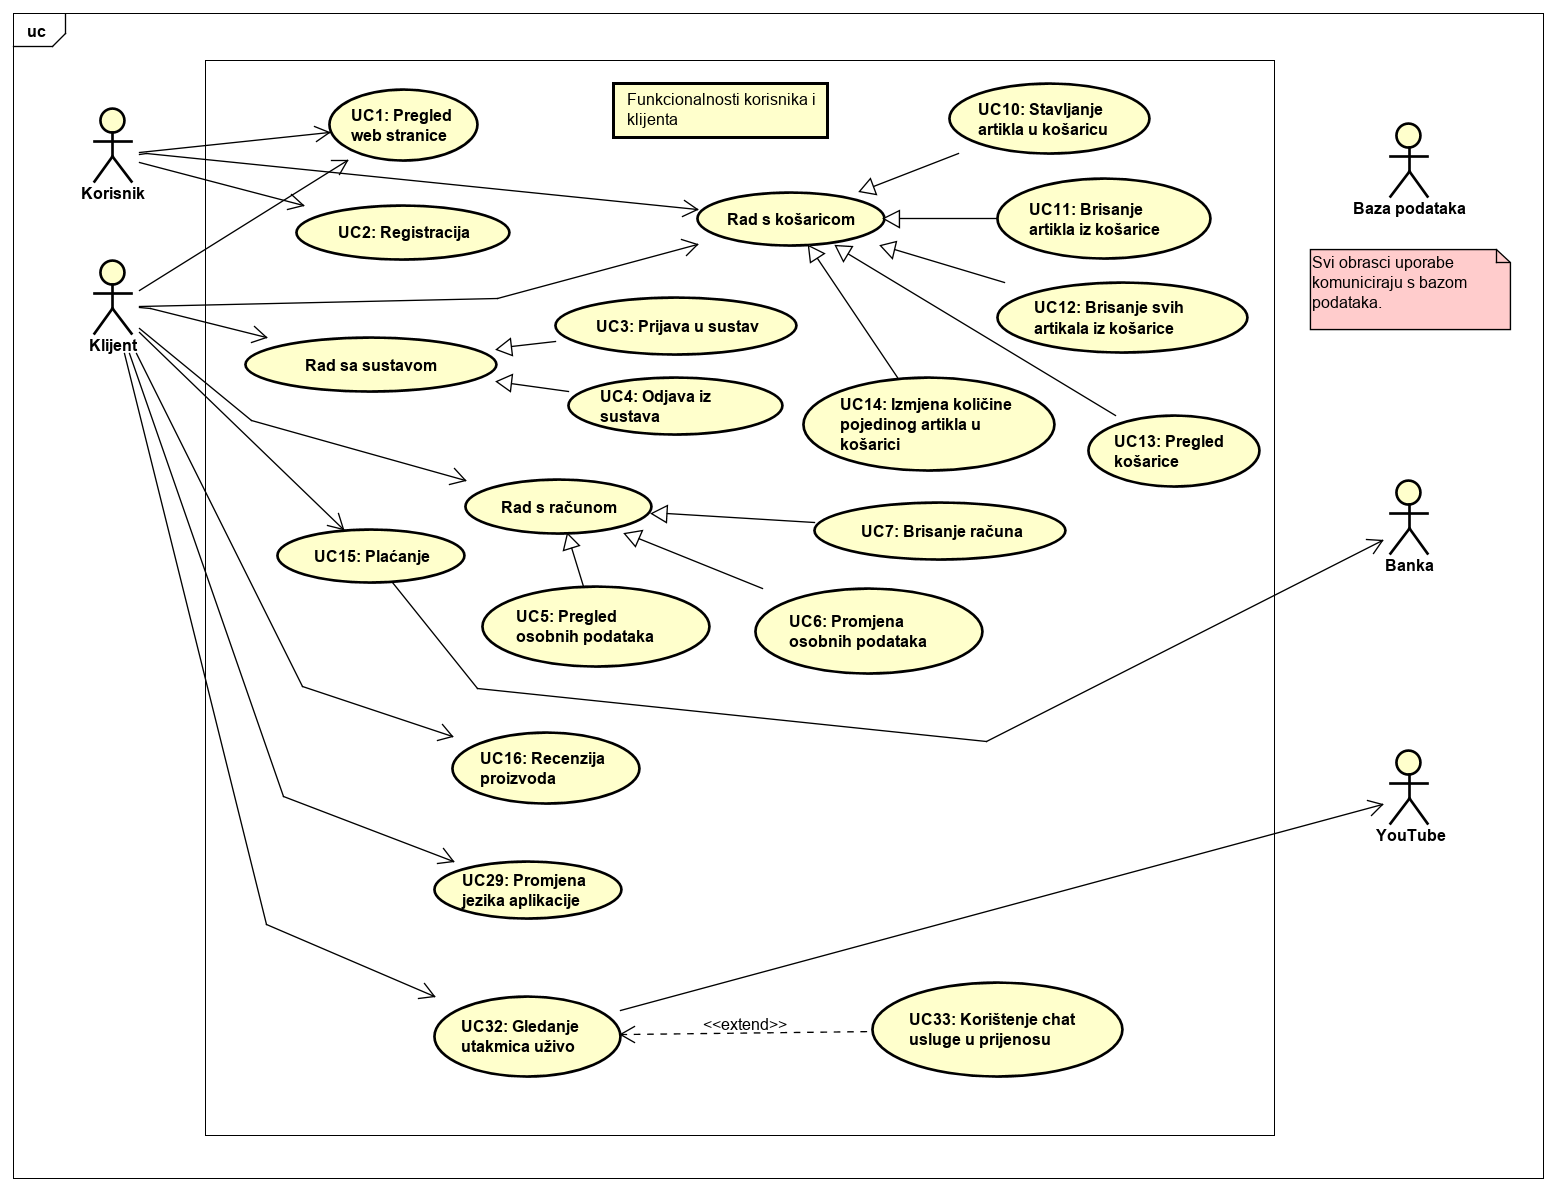
\includegraphics[width=\linewidth]{dijagrami/Funkcionalnosti_korisnika_i_klijenta.png}
						\centering
						\caption{Funkcionalnosti korisnika i klijenta}
						\label{fig:UseCaseDiagram1}
					\end{figure}
				
					\begin{figure}[H]
						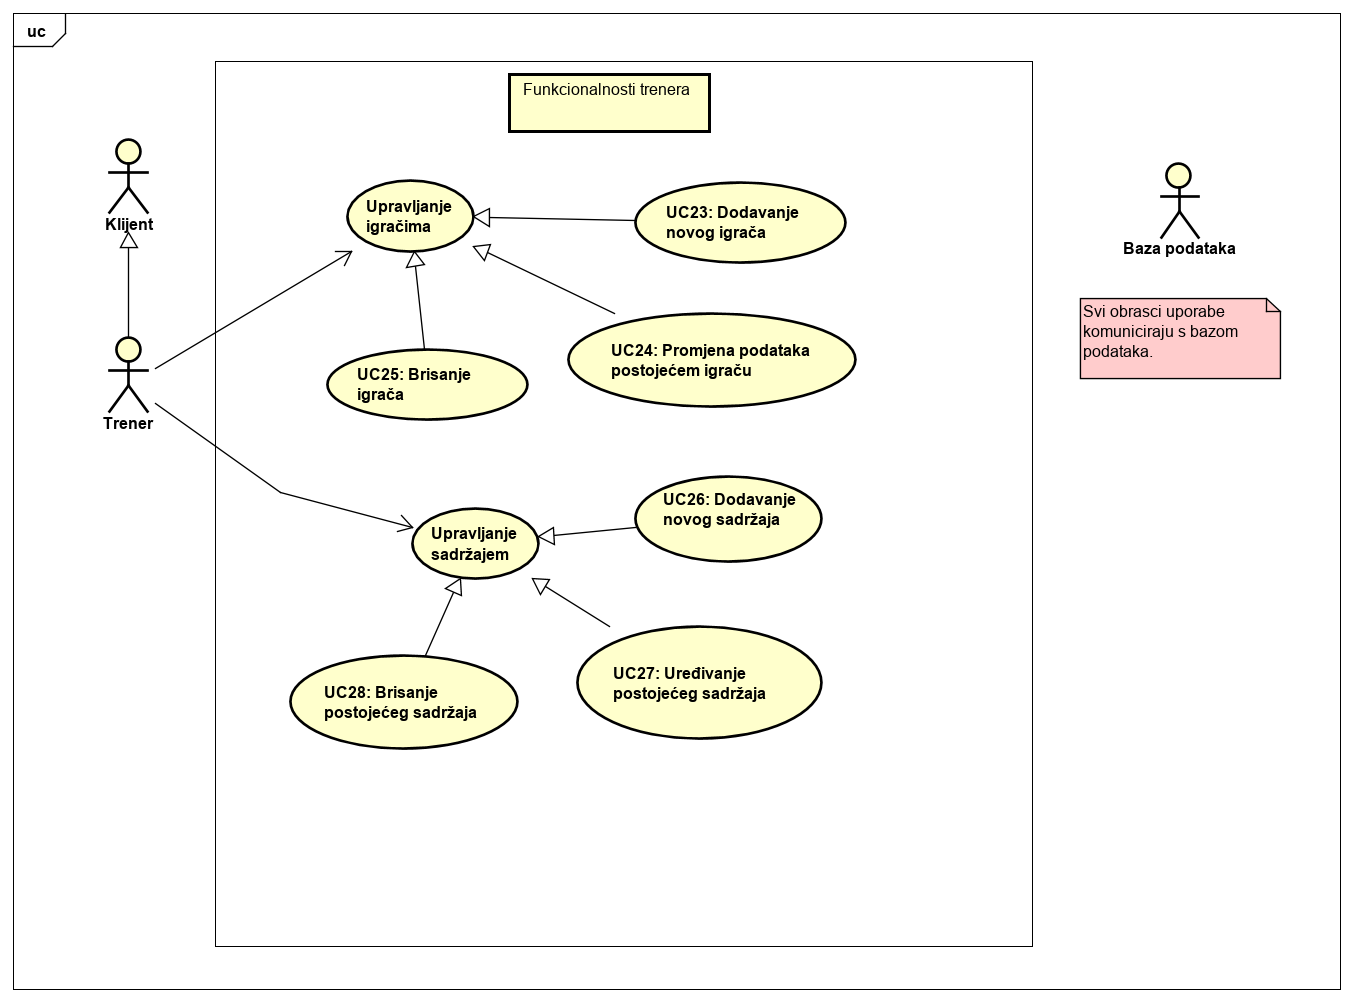
\includegraphics[width=\linewidth]{dijagrami/Funkcionalnosti_trenera.png}
						\centering
						\caption{Funkcionalnosti trenera}
						\label{fig:UseCaseDiagram2}
					\end{figure}
				
					\begin{figure}[H]
						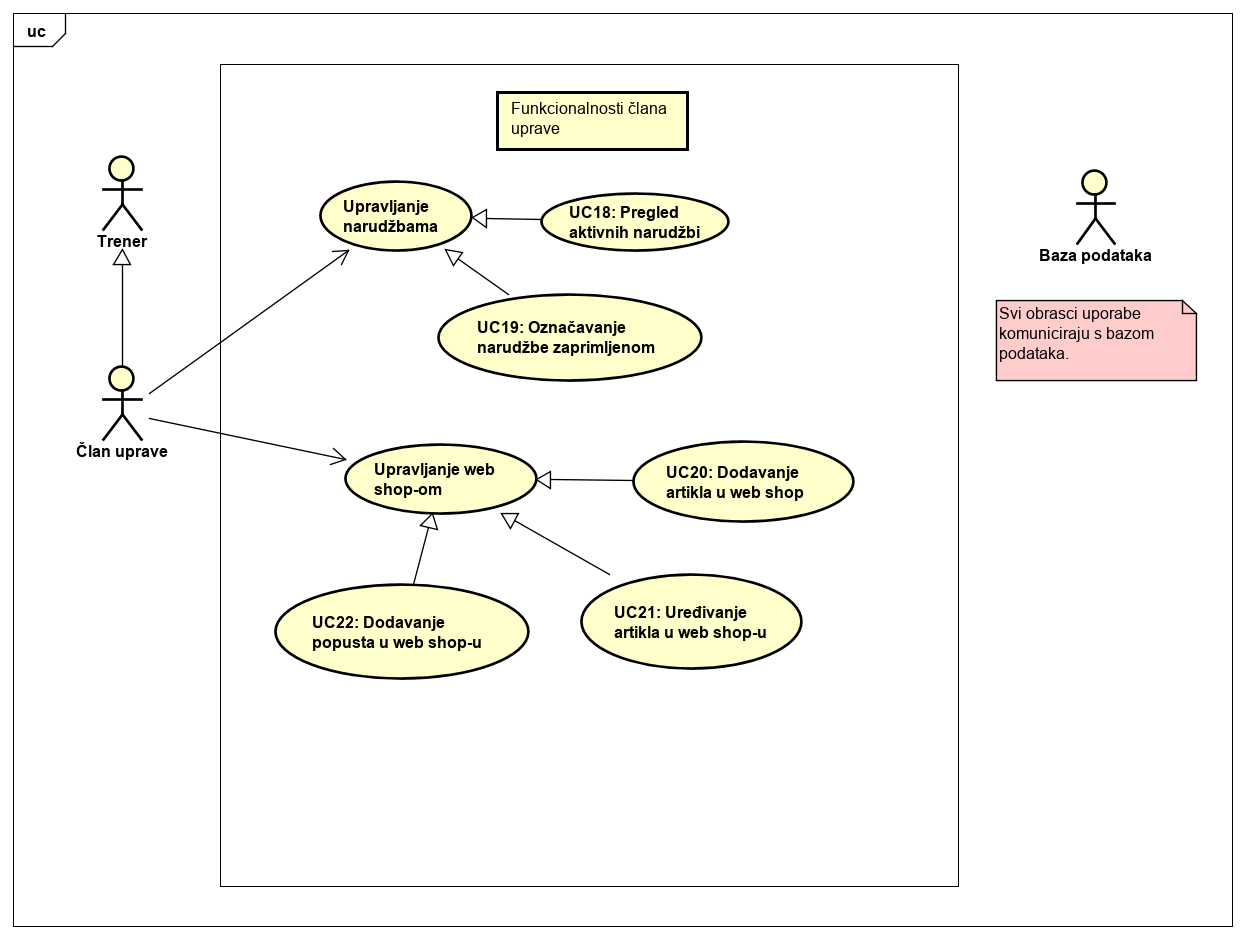
\includegraphics[width=\linewidth]{dijagrami/Funkcionalnosti_clana_uprave.png}
						\centering
						\caption{Funkcionalnosti člana uprave}
						\label{fig:UseCaseDiagram3}
					\end{figure}
				
					\begin{figure}[H]
						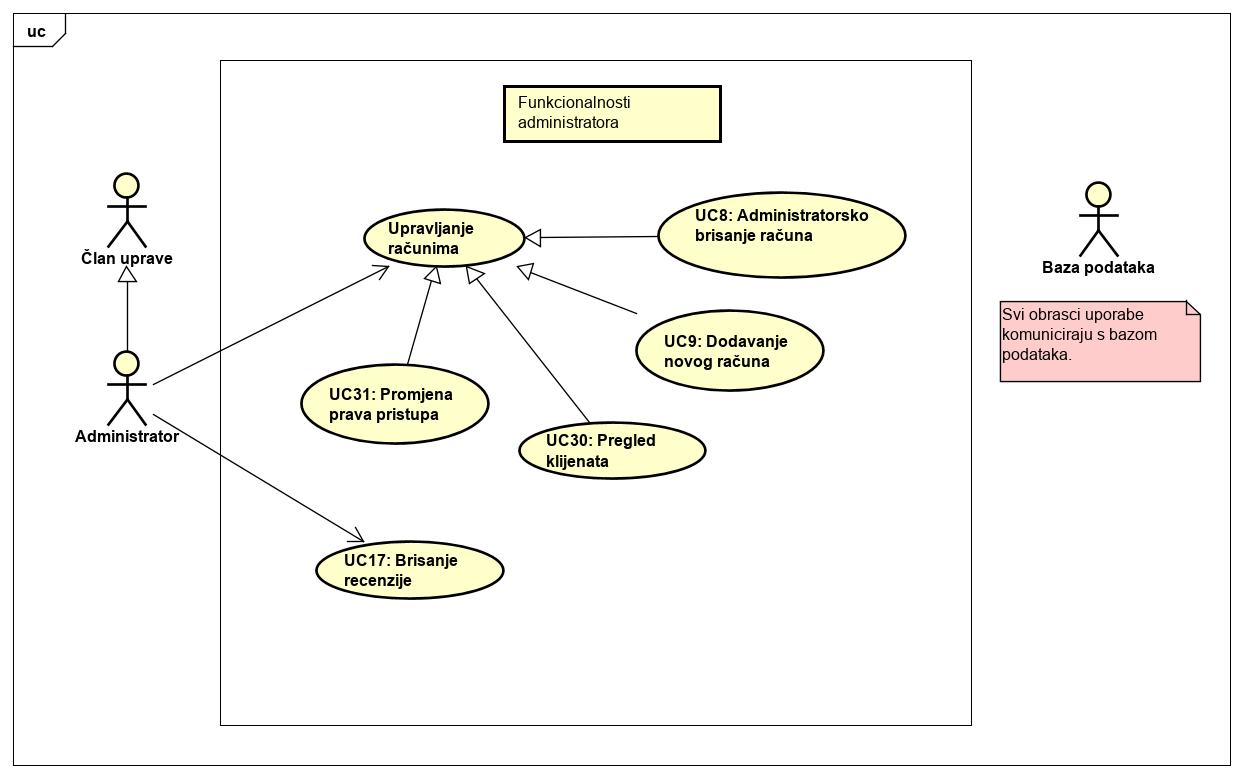
\includegraphics[width=\linewidth]{dijagrami/Funkcionalnosti_administratora.png}
						\centering
						\caption{Funkcionalnosti administratora}
						\label{fig:UseCaseDiagram4}
					\end{figure}
				
				\eject		
				
			\subsection{Sekvencijski dijagrami}
				
				\textbf {Obrazac uporabe UC10: Stavljanje artikla u košaricu }
				\bigbreak
				\textnormal {Korisnik šalje zahtjev za prikaz web shop-a kako bi mogao pregledati artikle. Poslužitelj dohvaća popis artikala i vraća ih te ih prikazuje u web shop-u koji korisnik pregledava. Odabirom artikla, koje korisnik bira dok ne odabere sve željene proizvode, korisnik bira količinu i veličinu proizvoda. Poslužitelj provjerava dostupnost artikla s bazom podataka i vraća informacije o artiklu. Ukoliko je artikl dostupan, korisniku se ispisuje poruka da je artikl dostupan i on šalje zahtjev za dodavanjem u košaricu. Poslužitelj šalje bazi zahtjev za mijenjanje sadržaja košarice, odnosno dodavanja artikla te baza sprema promjene. Ukoliko artikl nije dostupan, korisniku se ispisuje poruka.}
				\begin{figure}[H]
					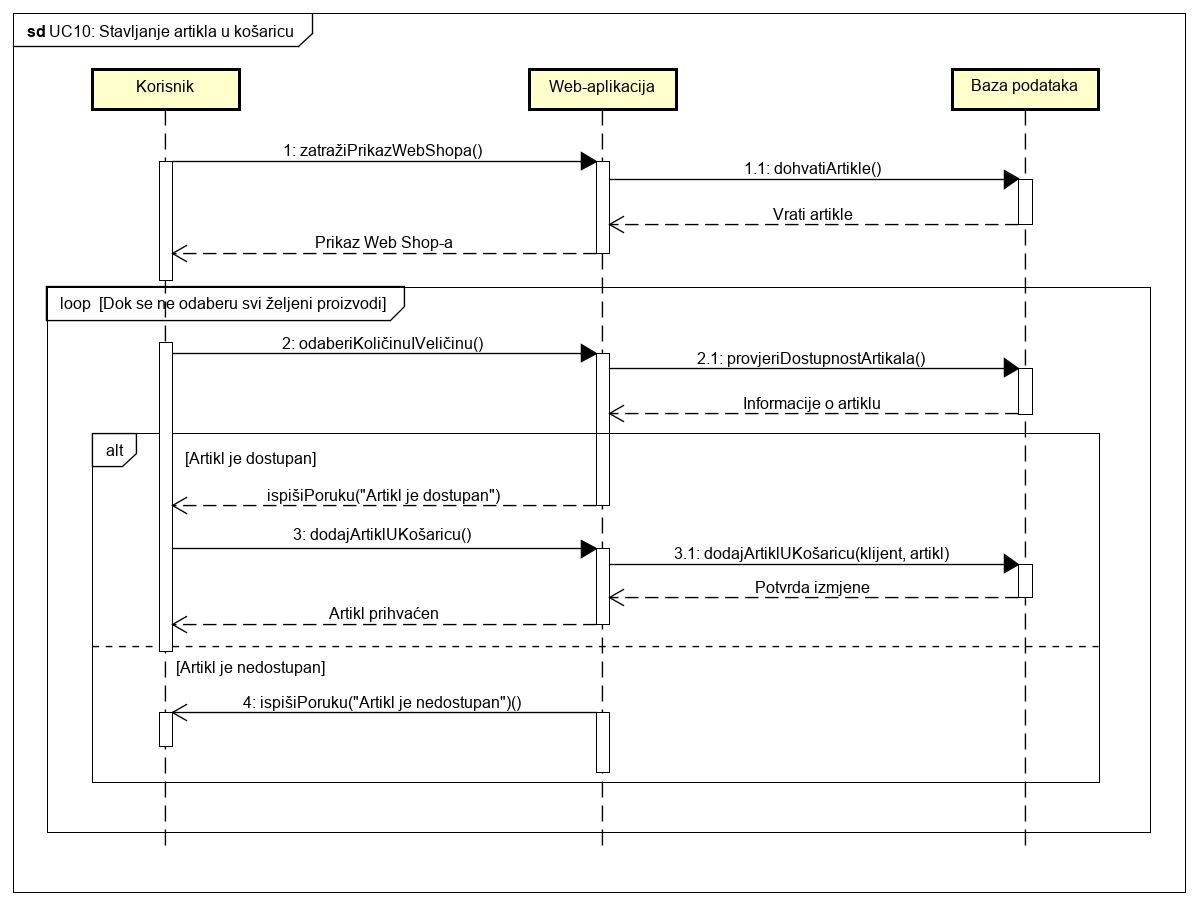
\includegraphics[width=\linewidth]{dijagrami/UC10.png}
					\centering
					\caption{UC10, Stavljanje artikla u košaricu}
					\label{fig:SequanceDiagram1}
				\end{figure}
			\bigskip
			\bigskip
			\bigskip
			
			\textbf {Obrazac uporabe UC15:Plaćanje}
			\bigbreak
			\textnormal {Klijent šalje zahtjev za pregled košarice kako bi mogao vidjeti odabrane artikle u košarici. Poslužitelj dohvaća sadržaj košarice iz baze te ga prikazuje klijentu. Klijent zatraži plaćanje te poslužitelj prikazuje formu za plaćanje koju klijent ispunjava te šalje nazad poslužitelju. Poslužitelj šalje banci zahtjev za transakcijom s određenim iznosom i karticom te banka vraća status transakcije poslužitelju. Na temelju statusa transakcije poslužitelj u bazi formira narudžbu i transakciju te isprazni košaricu. Ukoliko je transakcija odobrena, ispisuje se poruka korisniku. Ukoliko nije, također se ispisuje poruka o neuspješnoj transakciji.}
				\begin{figure}[H]
					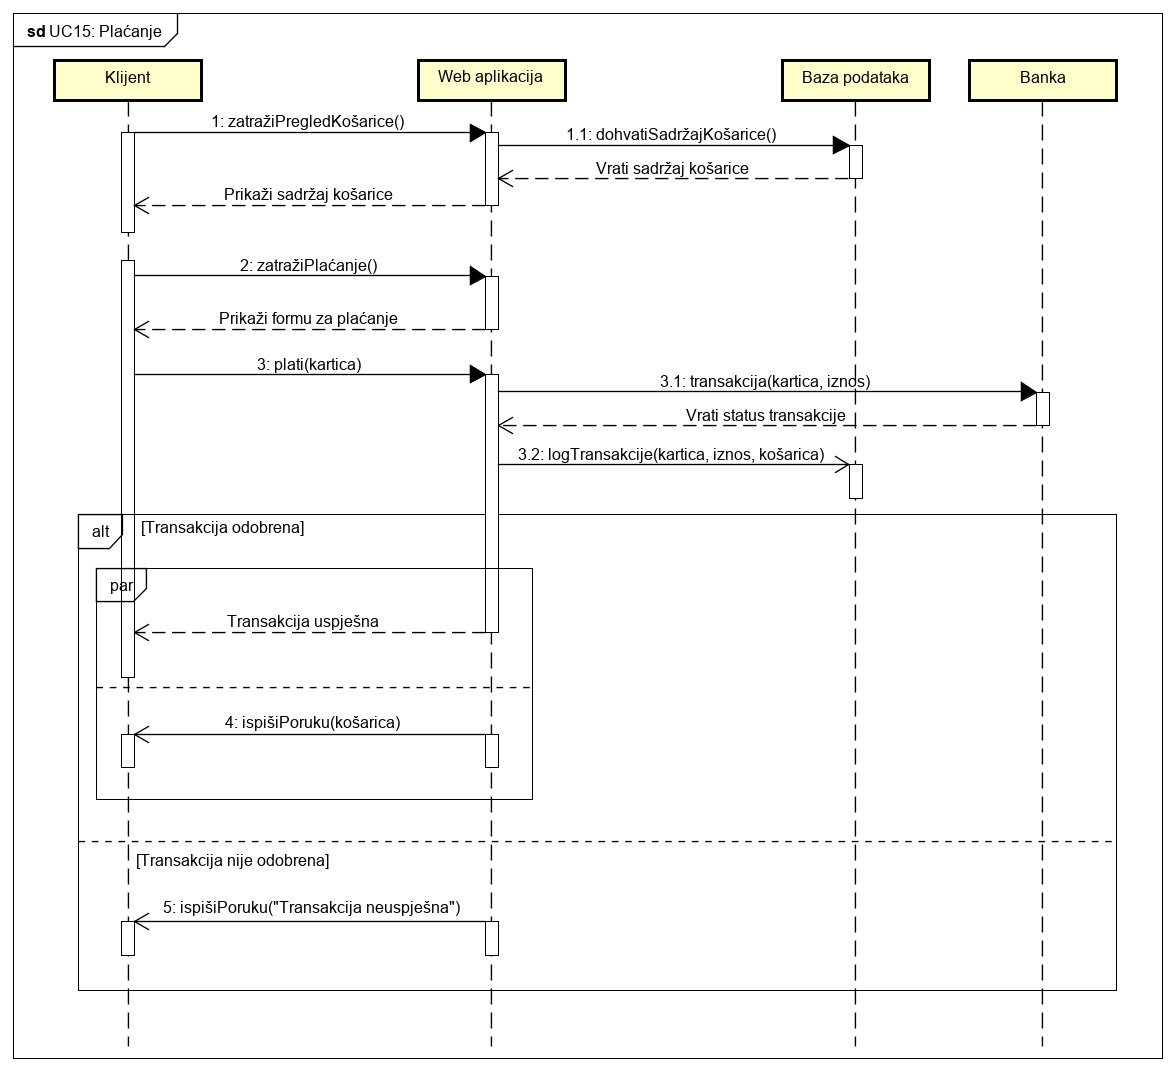
\includegraphics[width=\linewidth]{dijagrami/UC15.png}
					\centering
					\caption{UC15, Plaćanje}
					\label{fig:SequanceDiagram2}
				\end{figure}
			\bigskip
			\bigskip
			\textbf{Obrazac uporabe UC19: Označavanje narudžbe zaprimljenom}
			\bigbreak
			\textnormal {Član uprave zatraži listu aktivnih narudžbi koju poslužitelj proslijeđuje bazi te baza vraća listu aktivnih narudžbi poslužitelju. Ukoliko postoje aktivne narudžbe, poslužitelj ih prikazuje. Dok član uprave ne odabere sve narudžbe koje želi zaprimiti, šalje zahtjev za označavanje narudžbe zaprimljenom poslužitelju koji ih proslijeđuje bazi. Baza zatim potvrđuje izmjene i poslužitelj javlja da su promjene pohranjene. Ukoliko ne postoje aktivne narudžbe, poslužitelj ispisuje odgovarajuću poruku članu uprave.
			}
				\begin{figure}[H]
					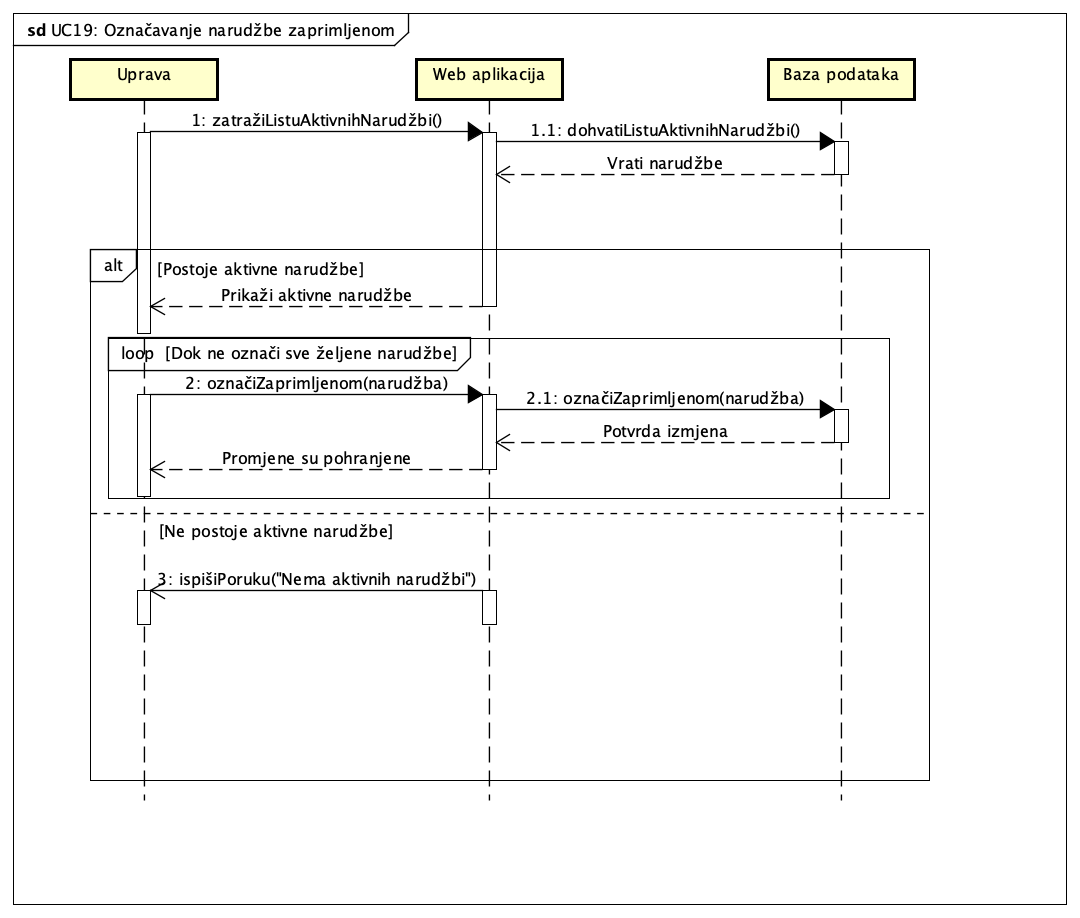
\includegraphics[width=\linewidth]{dijagrami/UC19.png}
					\centering
					\caption{UC19, Označavanje narudžbe gotovom}
					\label{fig:SequanceDiagram3}
				\end{figure}
			\textbf{Obrazac uporabe UC21: Uređivanje artikala u web shop-u}
			\bigbreak
			\textnormal {Član uprave šalje zahtjev za prikaz artikala koje poslužitelj dohvaća iz baze te ih prikazuje članu uprave. Član uprave odabere artikl, poslužitelj zatim šalje zahtjev bazi za njegov dohvat te baza vraća artikl koji se prikaže. Član uprave zatraži promjenu proizvoda sa starog na novi te poslužitelj vraća da je pristup odobren. Član uprave šalje promjenu proizvoda koju poslužitelj unosi u bazu podataka koja sprema promjene.}
				\begin{figure}[H]
					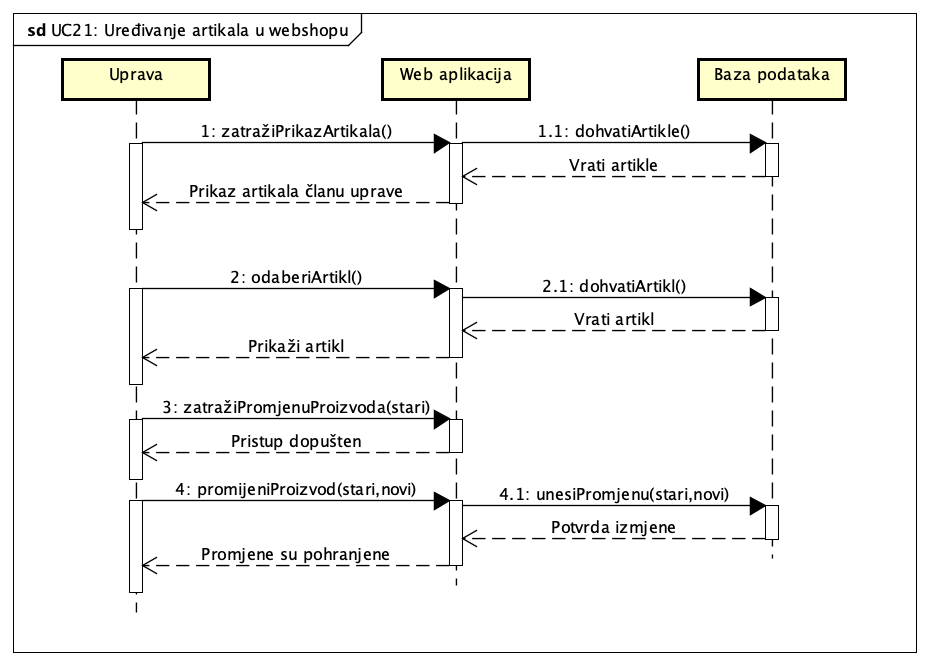
\includegraphics[width=\linewidth]{dijagrami/UC21.png}
					\centering
					\caption{UC21, Uređivanje artikala u web shopu}
					\label{fig:SequanceDiagram4}
				\end{figure}
	\eject
		\section{Ostali zahtjevi}
		
			\begin{packed_item}
				\item Sustav treba omogućiti rad više korisnika u stvarnom vremenu
				\item Korisničko sučelje i sustav moraju podržavati hrvatsku abecedu (dijakritičke znakove) pri unosu i prikazu tekstualnog sadržaja
				\item Izvršavanje dijela programa u kojem se pristupa bazi podataka ne smije trajati duže od nekoliko sekundi
				\item Sustav treba biti implementiran kao web aplikacija koristeći objektno-orijentirane jezike
				\item Neispravno korištenje korisničkog sučelja ne smije narušiti funkcionalnost i rad sustava
				\item Sustav treba biti jednostavan za korištenje, korisnici se moraju znati koristiti sučeljem bez opširnih uputa
				\item Nadogradnja sustava ne smije narušavati postojeće funkcionalnosti sustava
				\item Sustav kao valutu koristi HRK
				\item Veza s bazom podataka mora biti kvalitetno zaštićena, brza i otporna na vanjske greške
				\item Front-end web aplikacije bit će implementiran uz pomoć HTML5, CSS3, Bootstrap 4 i Vue.js tehnologija
				\item Back-end web aplikacije bit će implementiran u programskom jeziku C\#
				\item Čitav sustav će biti utemeljen na okviru rada ASP.NET Core 3.0
				\item Sustav će podržavati hrvatski i engleski jezik
			\end{packed_item}

			 
			 
			 
	